% !TEX root = main.tex

For right now, we will be setting the Radon Transform aside. \\

We need to work on solving:

\begin{align*}
\widehat{\vec{q}}_{,t} + \widetilde{\mat{A}}(\omega) \widehat{\vec{q}}_{,s} = \vec{0} \\
\widehat{\vec{q}}_{,t} + \widetilde{\mat{A}}\,\widehat{\vec{q}}_{,s} = \vec{0}
\end{align*}

We will be picking one value for $\omega$ so that we can figure out how to solve this first, therefore using the second equation. \\

There are two key ingredients to solving this: \\
1. We need to know how to discretize in time, which is sometimes called time-stepping. \\
2. We need to know how to discretize in "space" ("space" being our s variable)
We will be starting with discretizing "space".
In order to do this, we need to replace $\frac{\partial}{\partial s}$ by a discrete matrix $\mat{D}$ \\

An example of this is the Central Finite Differences for $\widehat{\vec{q}}_{,s}$: \\

\begin{align*}
\widehat{q}(s)\ms\lra\ms\widehat{\vec{Q}} =  [\,\widehat{q}(s_1)\ms,\ms\widehat{q}(s_2)\ms,\ms\widehat{q}(s_3)\ss.\ss.\ss.\ss]
\end{align*}

When working with a fixed time interval, we have a mesh with an even grid spacing.

\begin{figure}[H]
\centering
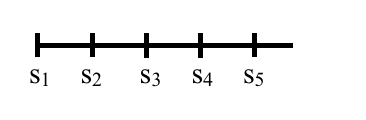
\includegraphics[width=0.25\textwidth]{MeshLine.jpg}
\caption{In the graphic above, the distance between the points is h units apart. This makes the graphic a uniform mesh.}
\end{figure}

To roughly discretize in space, we will use Central Finite Differences. 

\begin{align*}
\widehat{q}_{,s} |_{s_k} \approx \frac{\widehat{Q}_{k+1} - \widehat{Q}_{k-1}}{2h}
\end{align*}

This creates a 3-point stencil with error $O(h^2)$. 

\begin{align*}
\widehat{q}_{,s} \approx \mat{D}\,\widehat{\vec{Q}} = \frac{1}{2h}* \begin{bmatrix} 0&1&  &  &0 \\ -1&0&1  &  & \\   &-1&0&\ddots  &  \\   &  &\ddots&\ddots&1 \\ 0&  &  &-1&0 \end{bmatrix} \begin{bmatrix} \widehat{Q}_1 \\ \widehat{Q}_2 \\ \vdots \\ \widehat{Q}_{N-1} \\ \widehat{Q}_N \end{bmatrix}
\end{align*}
This however, is not exact. When we use a stencil in this manner, we end up with slight issues that relate to the boundary conditions. For now, we will ignore this fact and focus on the middle portion that includes the $-1, 0, 1$ signature. We can even create wider stencils, like a 5-point stencil, which has error $O(h^4)$.

When we use wider and wider stencils, we can theoretically produce more accurate approximations of the derivative:
\begin{align*}
\text{3-point stencil}\,\,\,\,\,\,\,\, \text{error}\,O(h^2) \\
\text{5-point stencil}\,\,\,\,\,\,\,\, \text{error}\,O(h^4) \\
\vdots\,\,\,\,\,\,\,\,\,\,\,\,\,\,\,\,\,\,\,\,\,\,\,\,\,\,\,\,\,\,\,\, \\
2k+1\text{-point stencil}\,\,\,\,\,\,\,\, \text{error}\,O(h^{2k})
\end{align*}
For generic $\widehat{q}(s)$, you don't observe optimal $O(h^{2k})$ accuracy. In fact, $|| \,\mat{D}\,\widehat{\vec{Q}} - \widehat{q}_{,s}\, || \lra \infty$ as $h \lra 0$. This is called the Runge phenomenon. \\
The problem is that we used equally spaced points. 
"Optimal" points that would work better for what we need would be Chebychev points. 
\begin{align*}
s \in [-1,1] \\
s_j = \cos(j\pi/N) \\
N+1 \,\, points \\
j = 0, 1, 2, . . .  \\
s_0 = 1 \,\,\,\,
s_N = -1
\end{align*}
\begin{figure}[H]
\centering
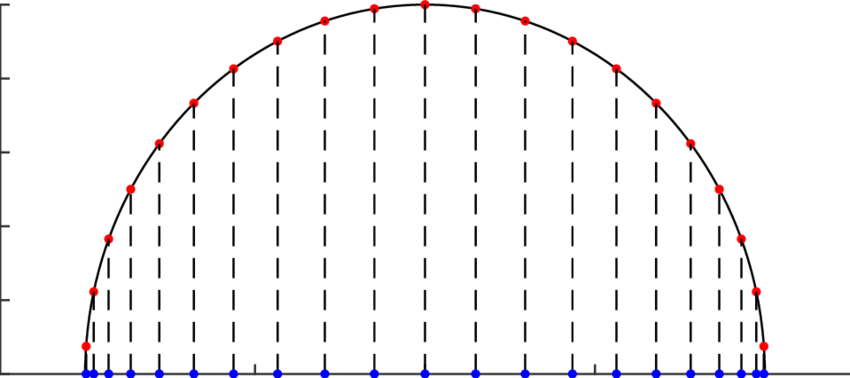
\includegraphics[width=0.8\textwidth]{ChebyshevPoints.jpg}
\caption{The above graphic has red dots to show the uniformly spaced points on the sine curve and blue dots to show the non-uniformly spaced Chebyshev points that will be used for our mesh.}
\end{figure}
The density of the grid points is high at the ends and low in the middle. Therefore, now we have a non-uniform mesh that has small spacing near $s = \rpm\,1$ and has large spacing near $s = 0$.\\
When we calculate the derivative at all points we get the following matrix. \\
\begin{figure}[H]
\centering
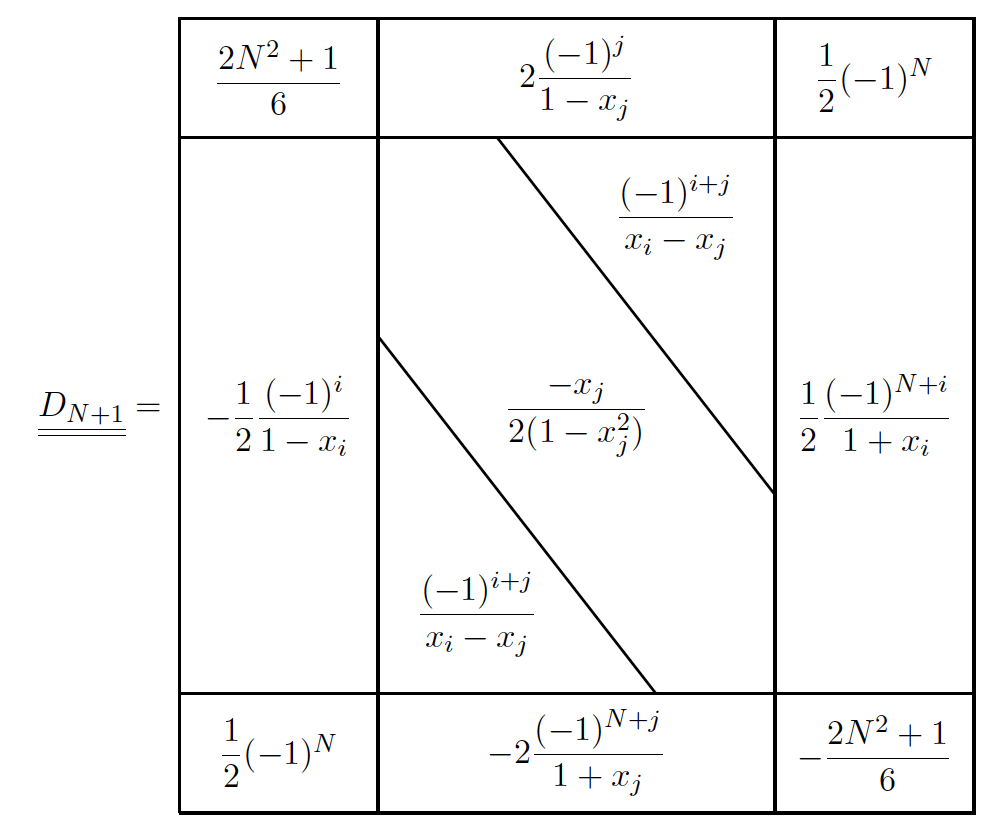
\includegraphics[width=0.8\textwidth]{Chebyshev.jpg}
\caption{This graph is from Spectral Methods in MATLab by Trefethen.}
\end{figure}
This is the Spectral Method. 